% 1章
\chapter{序論}
\label{chap:introduction}
%
%\input{introduction/preface}
%
%!TEX root = ../thesis.tex

\section{背景}
AIFormulaは計測自動制御学会と自動車技術会が主催し, 本田技術研究所がサポートする次世代の人工知能モビリティの競技会で, 正式な競技会は2025年から始まる.
AIFormulaは今後ますます需要が高まるであろう自動化システムの技術者を育てるという点で効果が見込まれる.
AIFormulaではハードウェアの変更もある程度許容されているが, 現時点での開発はソフトウェアが中心となる.
ハードウェアは経路追従するために必要なパーツが全て揃っているが, ソフトウェアはデバイスを駆動するサンプルプログラムが用意されているのみである.
競技という性質上, 経路追従などのソフトウェアは各チームで開発することが必要となる.
その点で, コースを自動で走行するためにはソフトウェアの開発は必須となる.

\subsection{ハードウェアとルール}
AIFormulaでは詳細なルールは検討中であるとのことで, 2025年2月に開催される予定のプレ大会以降に詳細なルールが決定される予定となっている.
Fig.1に2025年のプレ大会で使用されるロボットを示す.
プレ大会では指定されたコースを3周する時間で競われる.
LiDARなどは使用できないなど, いくつかの制約がある.

\begin{figure}[H]
  \centering
 \includegraphics[keepaspectratio, scale=0.6]
      {images/ExteriorViewOfTheMobilityPlatform.png}
 \caption{Exterior view of the mobility platform}
 \label{fig:robot view}
\end{figure}

\subsection{コース}
Fig.2にAIFormulaのコースを示す.
周囲に高い建造物のない平坦なコースである.


\begin{figure}[H]
  \centering
 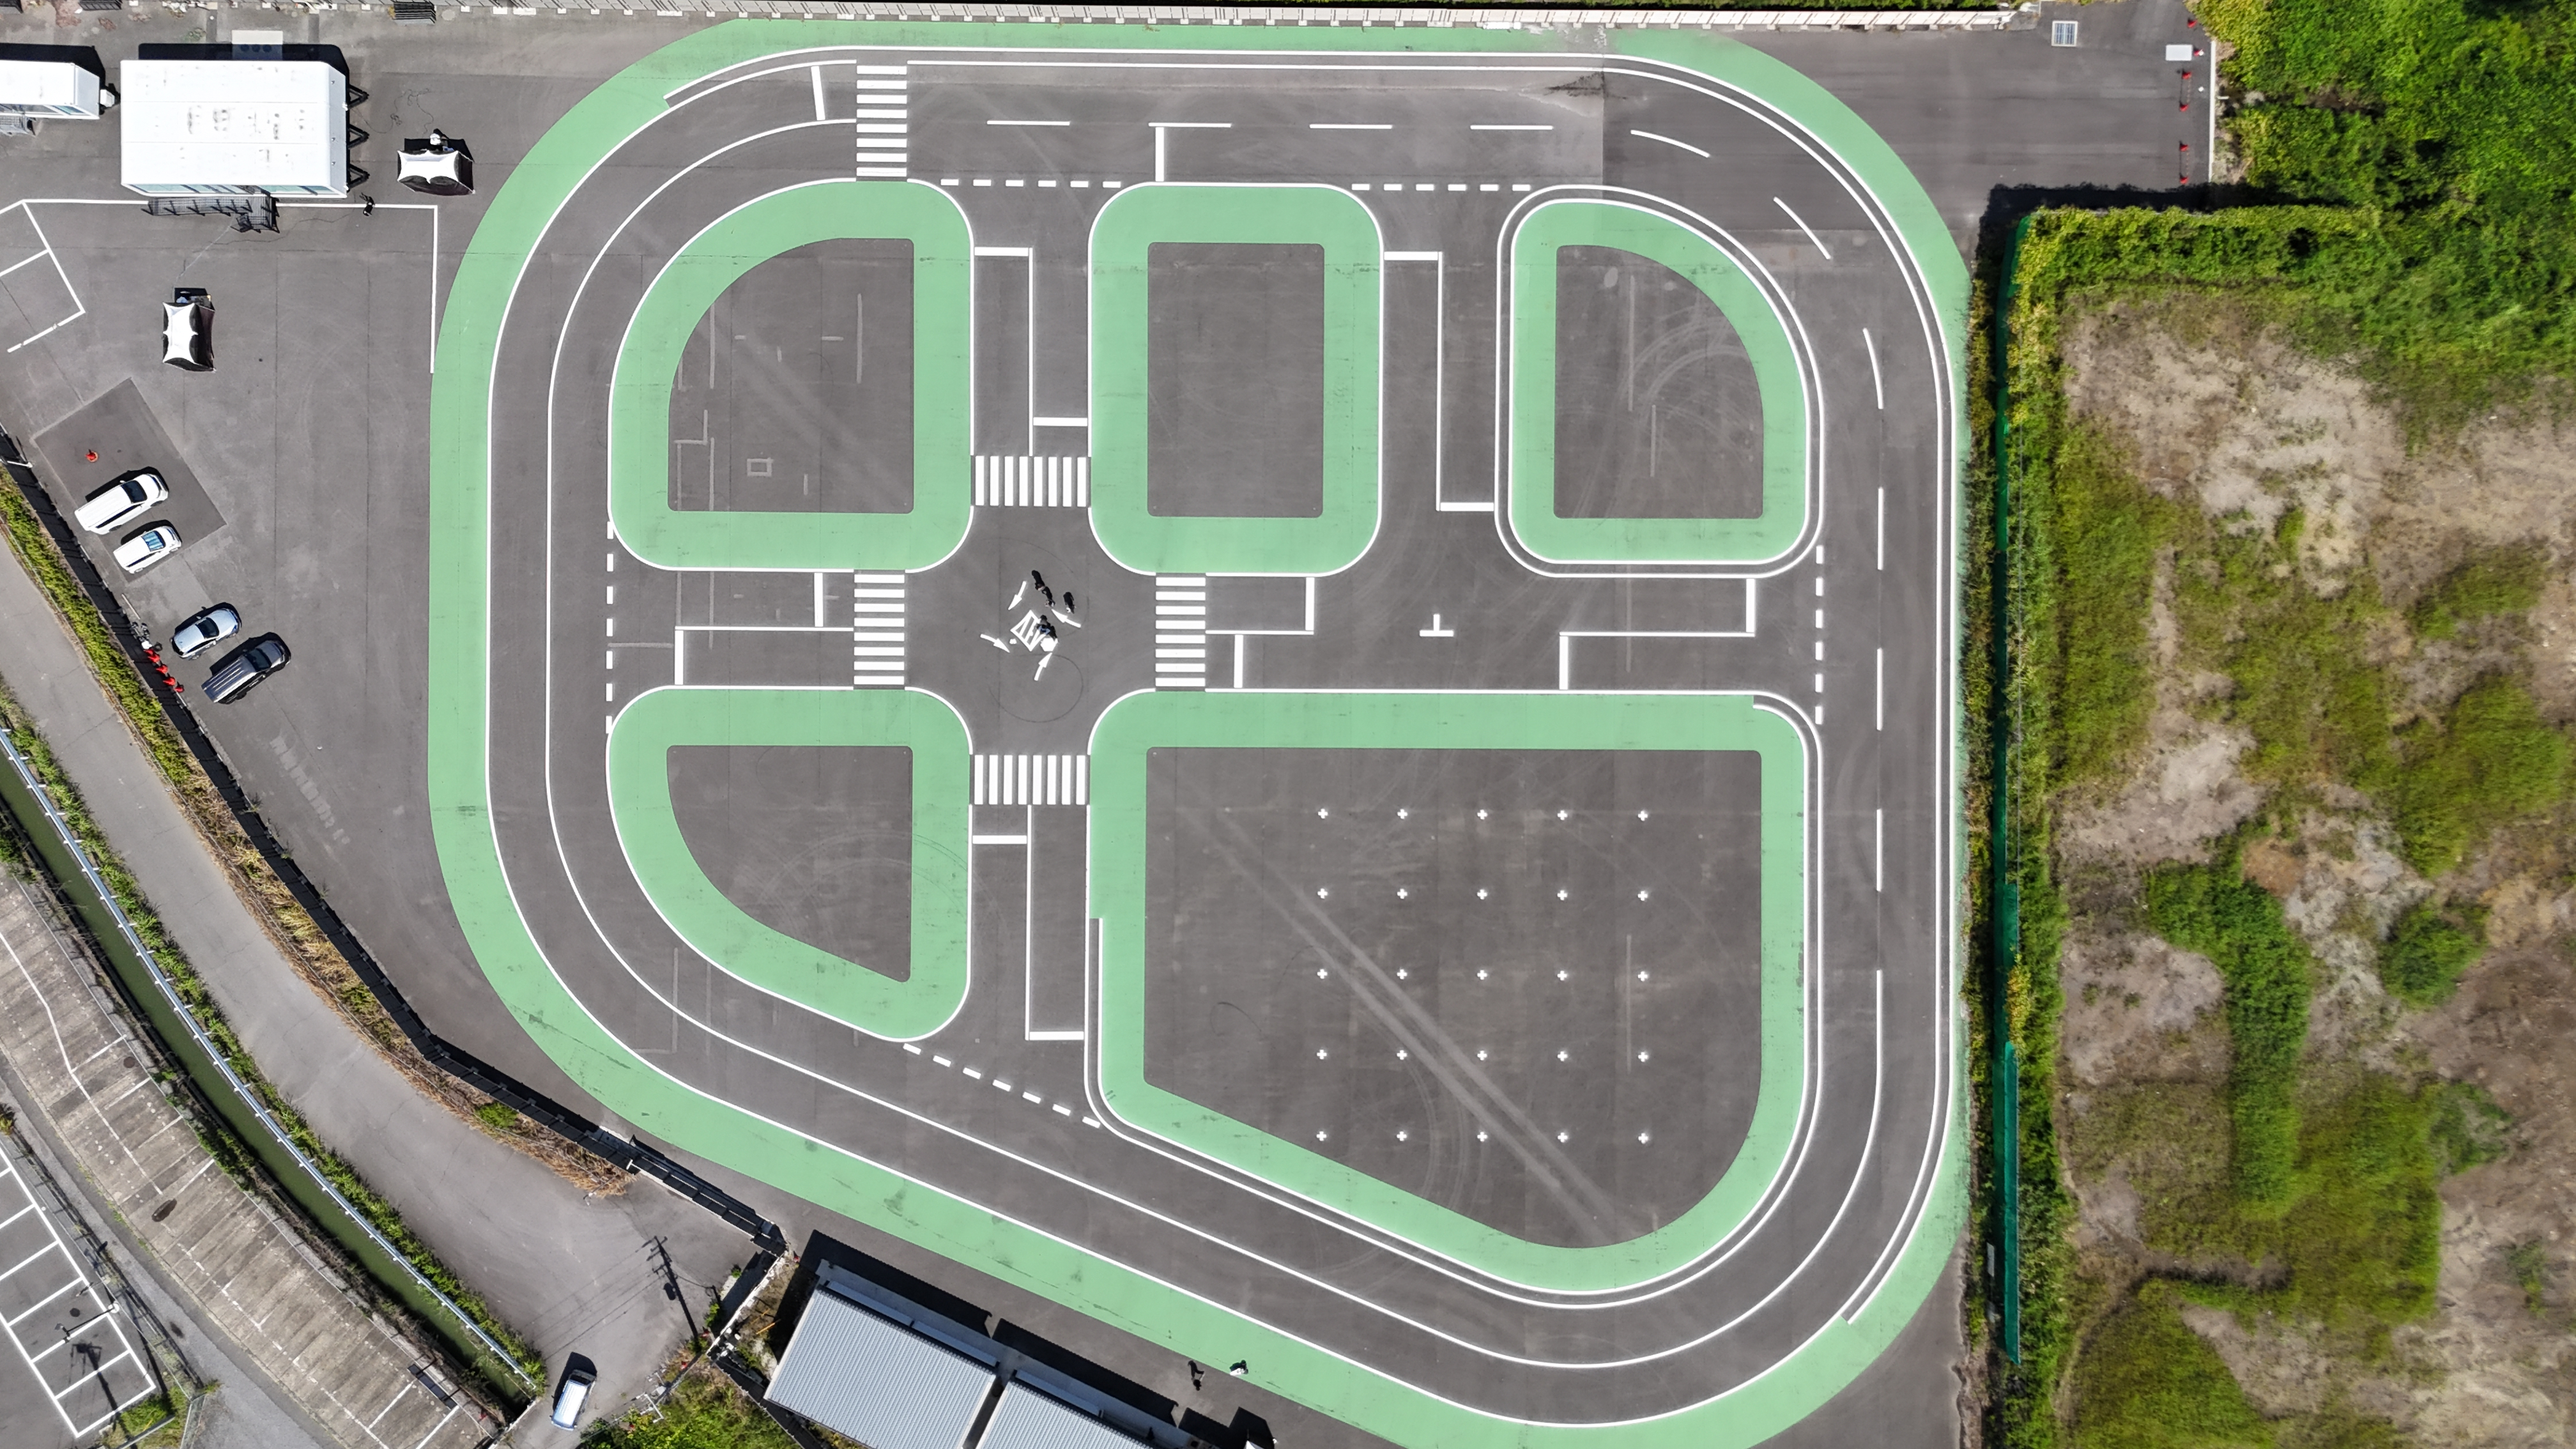
\includegraphics[keepaspectratio, scale=0.1]
      {images/AerialViewAndMobilitysPerspetiveOfTheCourse.png}
 \caption{Aerial view and mobility perspective of the course}
 \label{fig:course}
\end{figure}


\section{目的}
本研究では, 経路追従をするパッケージを開発して評価を行うことで作成した経路追従のパッケージの有効性を実環境で検証することを目的とする.


\section{論文の構成}
本論文は以下のように構成される.
まず, 2章で使用するセンサ構成とシステムの概要を示す.
3章では経路追従する際に使用するアルゴリズムについて述べる.
4章では開発したシステムを用いて経路追従をした際の追従性能の評価をおこなう.
5章では経路追従の実験結果をまとめる.

\newpage

% 2章
\chapter{要素技術}
本章では, 本研究に関連する要素技術を述べる.
%!TEX root = ../thesis.tex

\section{ROS 2}
ROS 2(Robot Operating System versition 2)は, オープンソースのロボットソフトウェアフレームワークであり,
ロボットアプリケーションの開発や実行をサポートするミドルウェアである.
異なるバージョンが存在しているが, 本研究ではROS 2 foxyを主に使用している.

\subsection{RViz2}
RViz2(ROS VIsualization2)はROS 2で提供される三次元ビジュアライゼーションツールであり, 
数値で表されるロボットの座標や各センサのデータを視覚的に表すことができる.

\section{GNSS}
GNSS(Global Navigation Satelite System)は, 
人工衛星を利用して地上の現在位置を計測するためのシステムであり, 
アメリカのGPS, ロシアのGLONASS, ヨーロッパのGalileo, 日本のQGSSなどを総称した衛生測位システムを指す.

\subsection{UTM座標系}
UTM(Universal Transverse Mercator)座標系とは, 全世界を経度6度ごとのゾーンに分けて東回りに番号を付けて規格化したものである.
世界的にも大・中縮尺の図法として採用され, 日本では国土地理院の地形図や地勢図で採用されている.

\begin{figure}[H]
  \centering
 \includegraphics[keepaspectratio, scale=0.7]
      {images/UTMCoordinateSystem.png}
 \caption{UTM Coordinate System(source)}
 \label{fig:purepursuit}
\end{figure}

% AIFormulaの会場となるAIモビリティパークは茨城県常総市にあるため, 54帯のUTM座標系を使用する.

\subsection{ECEF座標系}
ECEF(Earth-Centered, Earth-Fixed)座標系とは, 地理的・直交的な座標系であり, 地球の自転と同期して常時回転している座標系である.

\subsection{測地座標系}
測地座標系とは, 地球上の位置を緯度, 経度, および回転楕円体からの高さで表す座標系である.

\section{IMU}
IMU(Inertial Measurement Unit)は, 
3次元の慣性運動を検出する装置である. 
加速度センサーにより並進運動を検出し, 
ジャイロセンサーにより回転運動を検出することができる.

\newpage
% 3章
\chapter{経路追従のシステム}
ここでは, 本論文のベースとなるシステムについて述べる.
%!TEX root = ../thesis.tex

\section{ハードウェア}
本研究では, 屋外自律高速モビリティを制御対象とする.
モビリティは差動二輪と従動輪で構成された三輪モデルであり, 駆動モータの動作に追従するような従動輪機構となっている.
Fig.3.1に外装を取り付けたモビリティと外装を取り外したモビリティのハードウェアの外観を示す.

\begin{figure}[h]
     \centering
     \begin{minipage}[c]{65mm}
         \centering
         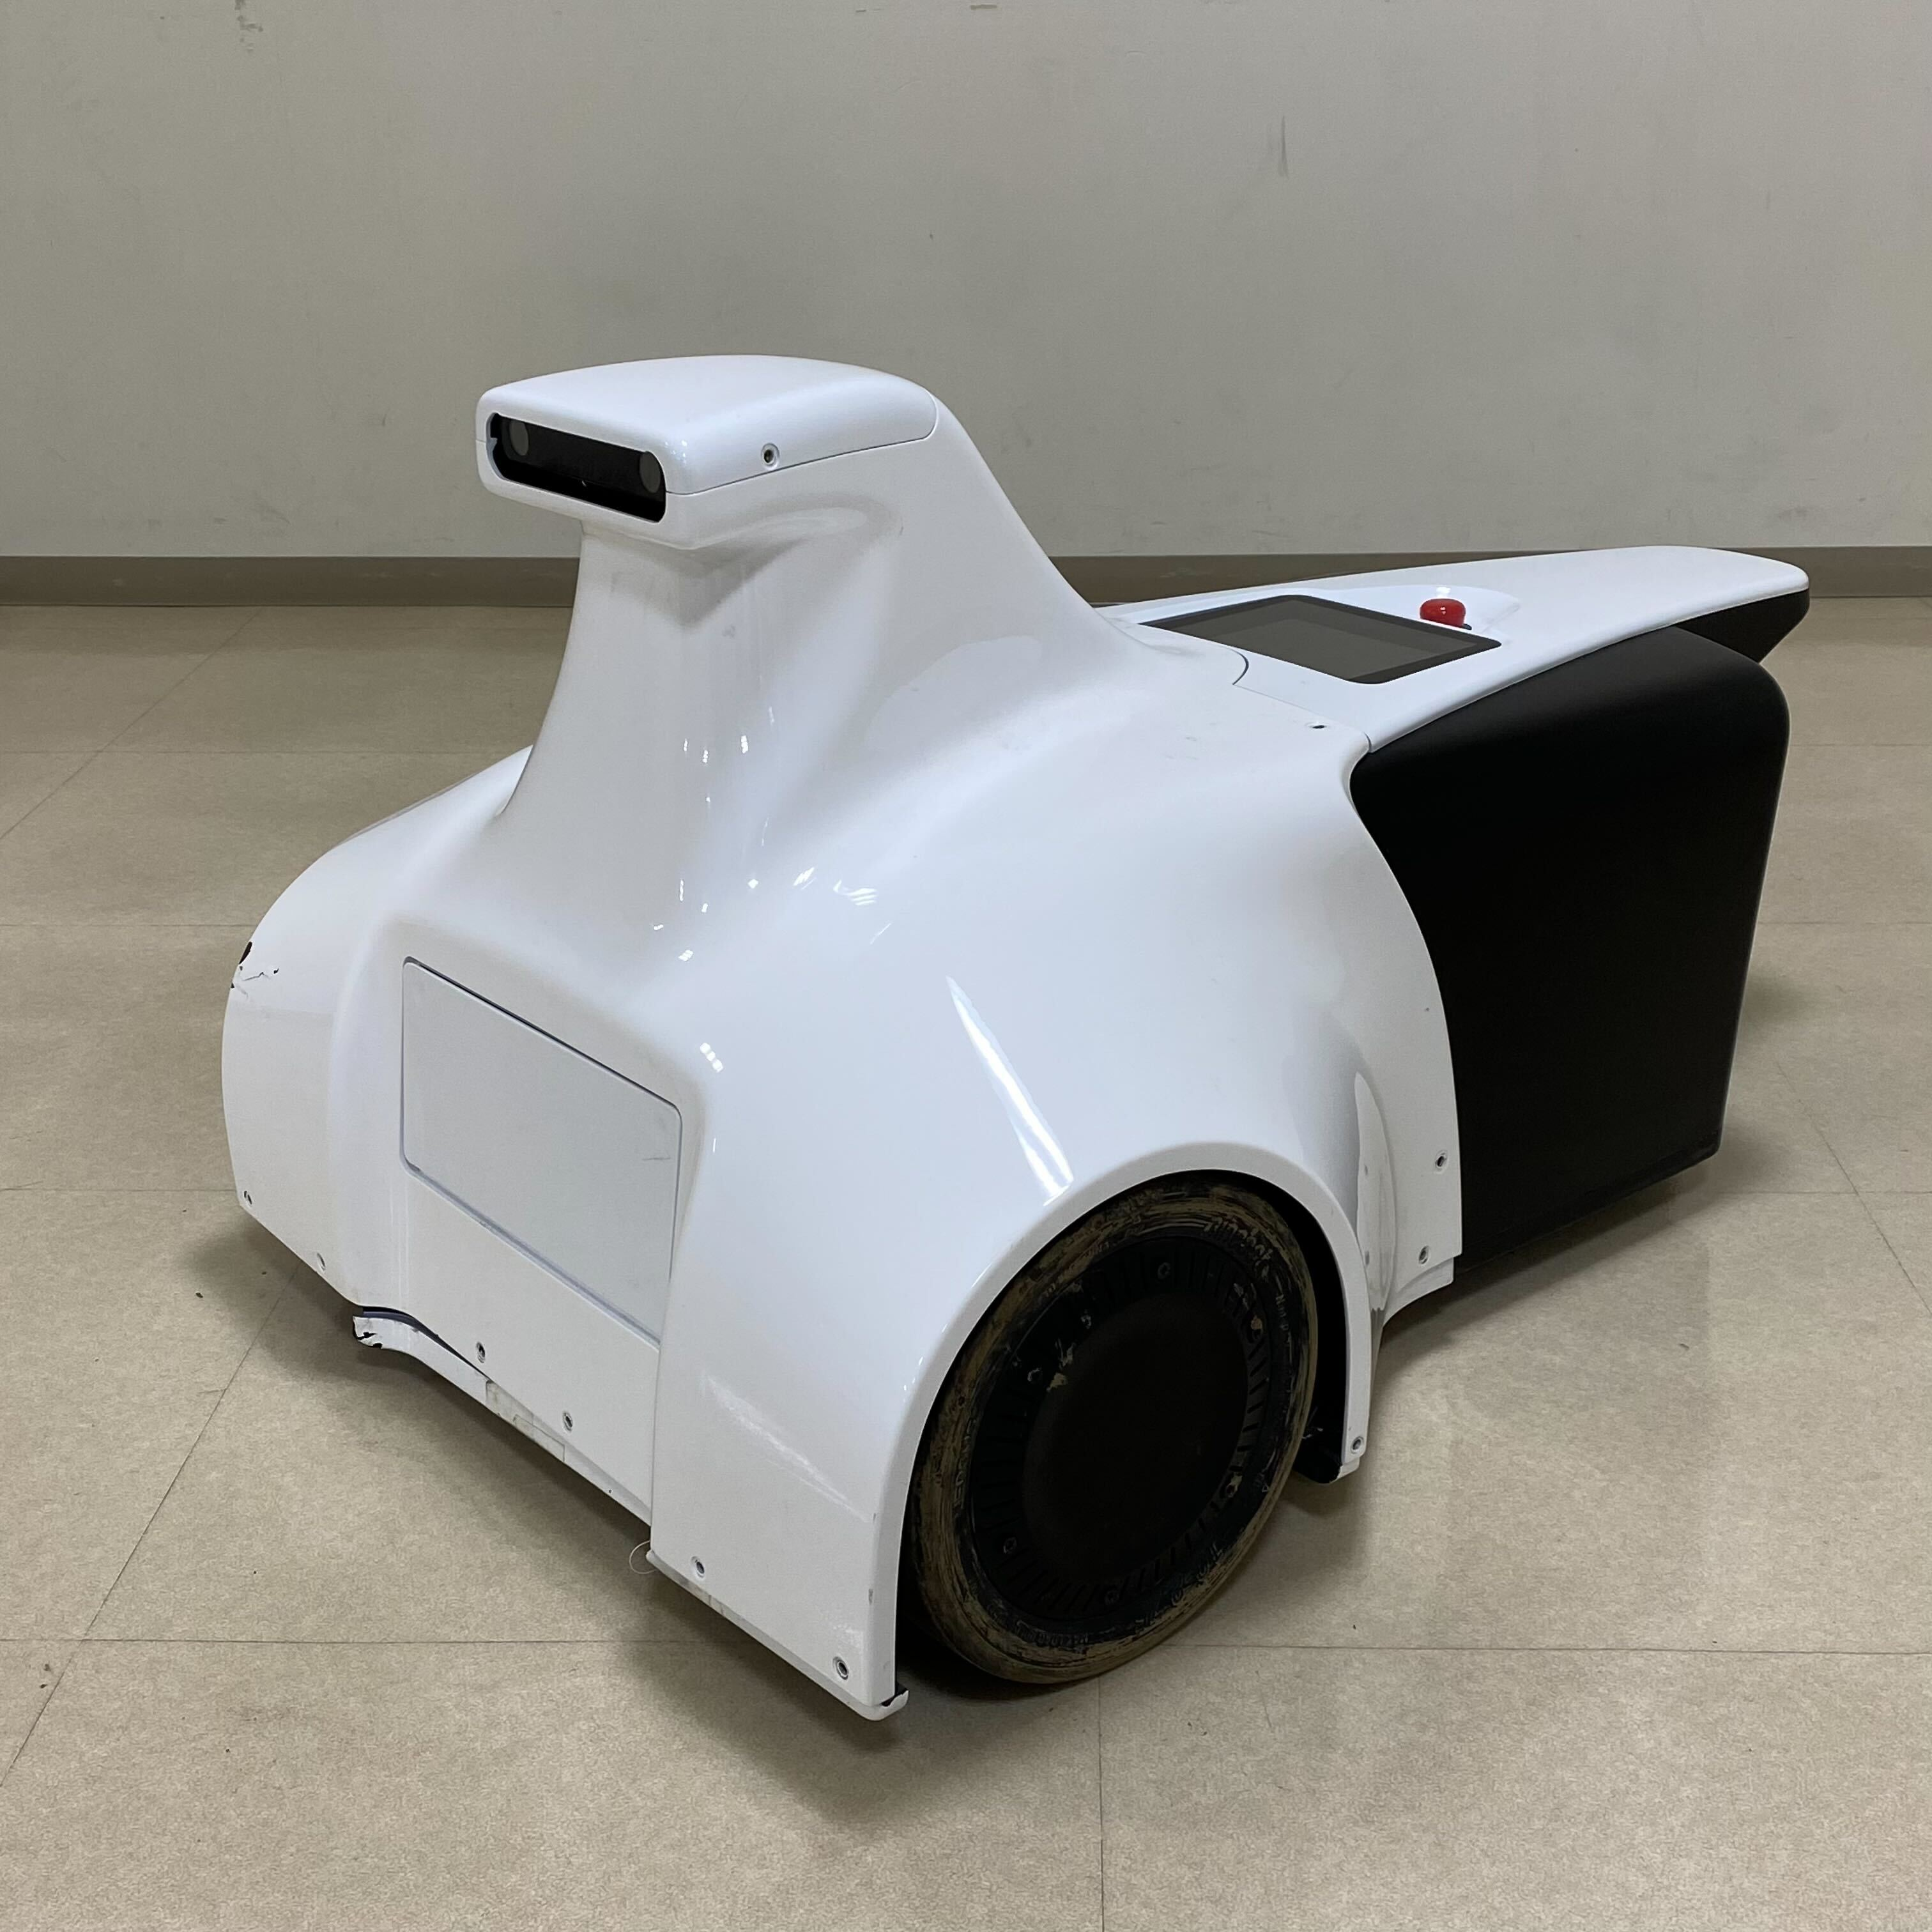
\includegraphics[height=50mm]{images/robotwithexterior.png}
         \subcaption{Mobility with exterior}
     \end{minipage}
     \begin{minipage}[c]{65mm}
         \centering
         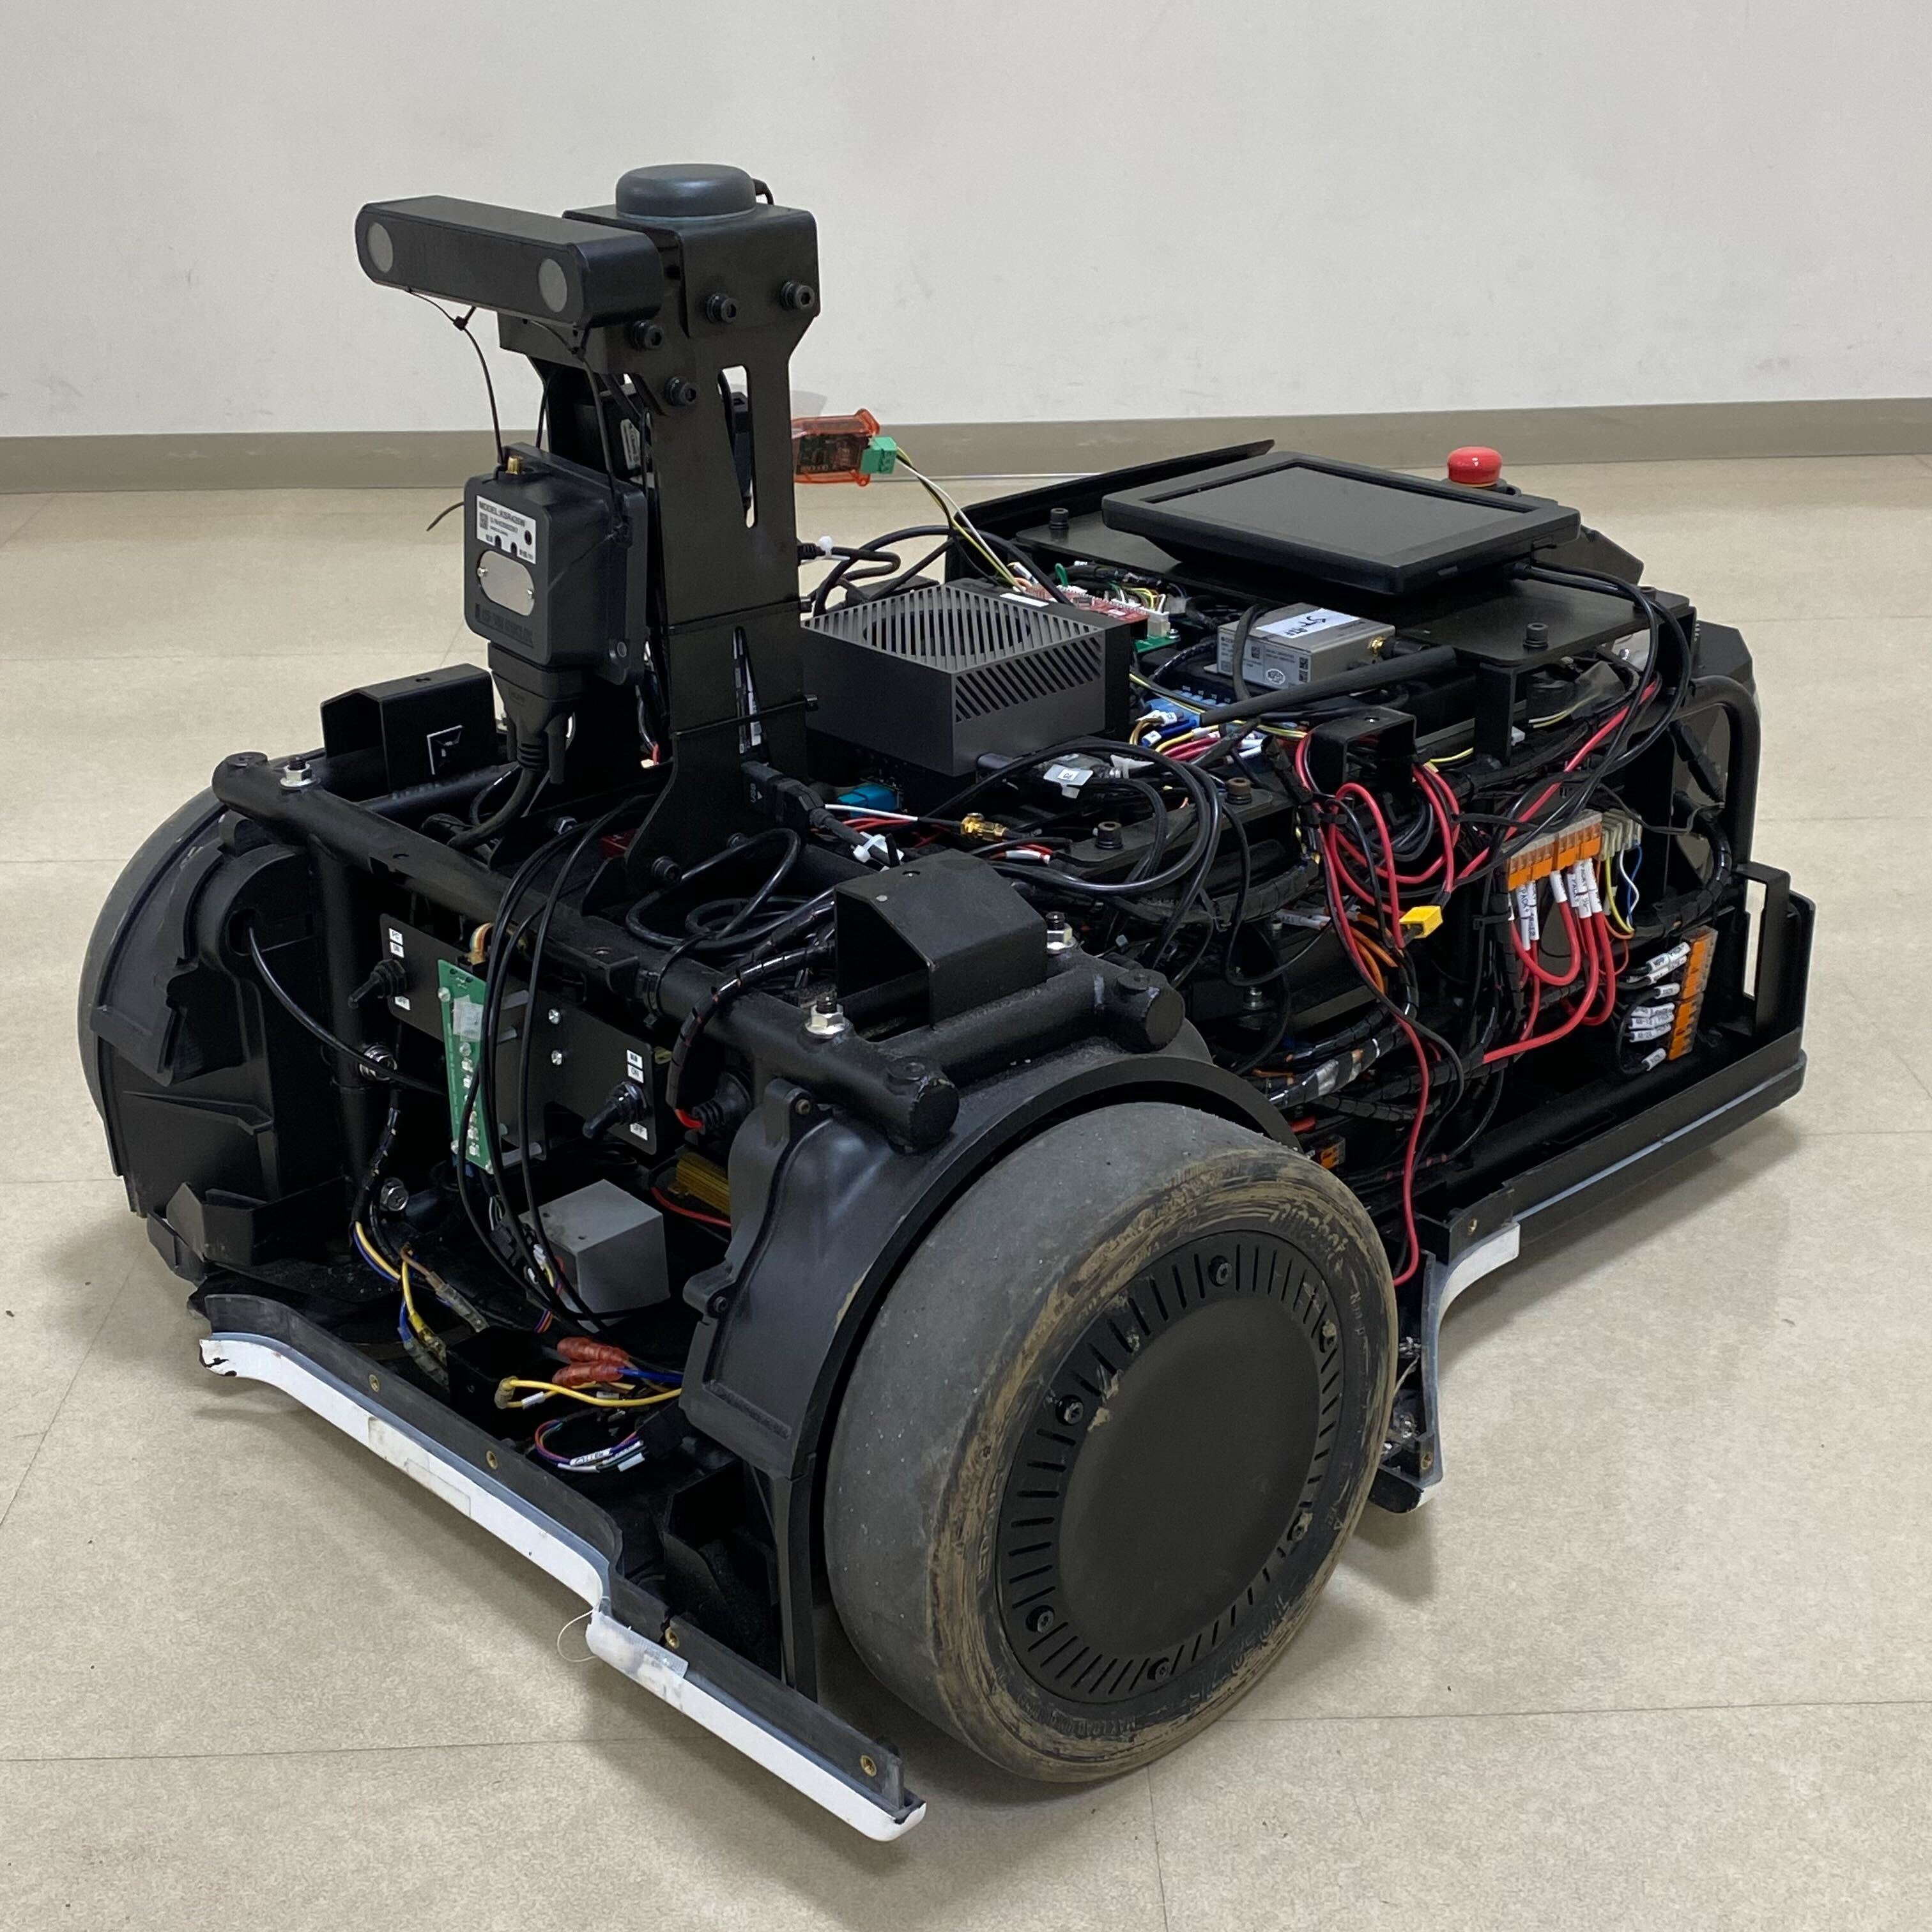
\includegraphics[height=50mm]{images/robotwithoutexterior.png}
         \subcaption{Mobility without exterior}
     \end{minipage}
     \caption{Robot appearance}
     \label{Fig:RobotGuidance_velocity}
\end{figure}

\subsection{センサ構成}
モビリティに搭載されているセンサ構成について述べる.
貸与されたモビリティにはステレオカメラ, GNSS+IMU, ホイールエンコーダなどのセンサが搭載されている.
開発するソフトウェアではGNSS+IMUセンサ(VectorNav VN-200)を使用する.

Fig.3.2にモビリティのセンサと位置を示す.

\begin{figure}[H]
     \centering
    \includegraphics[keepaspectratio, scale=0.7]
         {images/sensordescription.png}
    \caption{Mobility description}
    \label{fig:MPP}
\end{figure}

\subsubsection{VN-200}
VN-200\cite{vn-200}はGNSSとIMUを内包したセンサーであり, 3軸ジャイロ, 加速度計, 磁力系, GNSS受信機を用いて位置, 速度, 姿勢を推定することができる小型で高性能なGNSS支援慣性航法システムである.
IMUを内包しているため, 位置だけでなく方位も取得できるセンサとなっている.
VectorNavの方位は2種類の情報を手がかりに補正されるようになっており, 起動時は地磁気を手がかりに, 移動後はGNSSの履歴を手がかりに補正される.
ROS 2のラッパーとして, vectornavというパッケージが公開されている.\cite{vectornav}
Fig.3.3にVN-200の外観を示す.

\begin{figure}[H]
  \centering
 \includegraphics[keepaspectratio, scale=0.6]
      {images/vn-200.png}
 \caption{VectorNav VN-200 (source : [6])}
 \label{fig:vn-200 view}
\end{figure}

\subsection{従動輪}
貸与されたモビリティには従動輪の向きが望む方向に変化しない問題が発生していたため, 従動輪の向きをモータで駆動することで対処した.
これを実装したモビリティは結果的に, 高い操縦性により望む方向に移動できるようになった.
Fig.3.4に機構を示す.

% \phi= \arcsin\left(\frac{W\omega}{v}\right)

\begin{figure}[H]
  \centering
 \includegraphics[keepaspectratio, scale=0.5]
      {images/caster.png}
 \caption{Mechanism for driving the caster orientation}
 \label{fig:Mechanism for driving the caster orientation}
\end{figure}

\subsection{ブレーキ機構}
ブレーキ機構にはディスクブレーキと回生ブレーキが使用されている.
ディスクブレーキ機構はステッピングモータでディスクブレーキのワイヤを引っ張ることでブレーキがかかる機構となっている.

% \section{システム構成}
% ここで, 経路追従に用いることができるセンサはステレオカメラに加えてGNSSがある.
% 2つのセンサを比べたとき, 扱いの用意さという点ではGNSSに軍配があがる.
% ただし, マルチパスなどによる経緯度の誤差は数10mにおよぶことがあるため, 必ずしも経路追従に利用できるとは限らない.
% 幸いにして, AIFormulaの会場であるAIモビリティパークの周囲には高い建物が無く, マルチパスの影響が少ないと考えられた.
% そのため, GNSSに基づいた経路追従を行うシステムを開発した.
% Fig.4.4に経路追従で使用するシステム構成を示す.

% \begin{figure}[H]
%   \centering
%  \includegraphics[keepaspectratio, scale=0.2]
%       {images/system.png}
%  \caption{Path following system}
%  \label{fig:system}
% \end{figure}

% GNSSを用いて経路追従を行うためには, 位置に加えて方向のデータも必要となる.
% モビリティに搭載されているGNSS+IMU(VectorNav VN-200)は方位も計測できる仕様であるため, それを利用することが開発の多重化を防ぐ意味で望ましいと判断した.
% GNSS+IMU(VectorNav VN-200)はvectornav\cite{vectornav}というパッケージが公開されているため, そちらを使用してVectornavのセンサデータをROS 2 topicとして扱っている.
% 作成した経路追従のソフトウェアは, 事前にシュミレータ環境や手動走行をさせた時のGNSSから得た座標データをCSVファイルに経路情報としてまとめている.
% 用意した経路情報は測地座標系でまとめられていて, プロセスを起動したときにUTM座標系に変換されて目標経路の情報を含んだROS 2 topicとしてpublishされる.
% 経路追従を行うに際して, 自己位置はGNSSから取得した座標データをそのまま自己位置として扱っている.
% 取得した座標系はECEF座標系で取得されるため, 目標経路の座標系と合わせるためにUTM座標系に変換する.
% UTM座標系に合わされた目標経路の座標と自己位置の座標を利用してPurePursuitによる経路追従を行う.
% PurePursuitによって目標地点との角度差を取得し, その角度差に対してPID制御を行うことでモビリティの角速度を決定する.
% 並進速度は一定として, 求めた角速度に基づいてモビリティを制御する.

% \section{目標経路の作成}
% 経路追従をする際には追従するための目標経路が必要となる.
% 本研究では, 以下の図に示すように予め取得した経緯度のウェイポイントをつなぐライン状を移動する目標位置をPurePursuitで求め, 求めた目標地点に向かって進む制御を採用した.
% 経路情報はシミュレータ環境や事前に手動走行させたときのGNSSから得た情報を参照している.
% Fig.4.5に作成した目標経路の例を示す.

% \begin{figure}[H]
%   \centering
%  \includegraphics[keepaspectratio, scale=0.3]
%       {images/targetpath.png}
%  \caption{Predefined target trajectory}
%  \label{fig:target path}
% \end{figure}

\newpage
% 4章
% 開発するソフトウェアという内容に作り変えても良いかも
\chapter{経路追従に用いるアルゴリズム}
本章では, 経路追従に用いるアルゴリズムについて述べる.
%!TEX root = ../thesis.tex

\section{経路追従}
経路追従(Path following)とは, 経路計画(Path planning)で引いた経路に対してモビリティが経路を追従できるようにモビリティを制御することである.
基本的にはモビリティのモデルと制御アルゴリズムを利用することで, 最終的にモビリティの入力値(ステアリング角度や並進速度)を計算することが目的となる.

\subsection{PurePursuit}
PurePursuitアルゴリズムは, 経路追従アルゴリズムの中で最も基礎的だが, 非常に広く使われているアルゴリズムである.

PurePursuitはFig.3.1に示すように目標経路上(Path)に対して一定距離先の点を目標点(Look Ahead)とし, その点に到達するようなステアリング制御を行う.
目標点に対してモビリティが前進することで, より先の目標点にたどり着くように制御を行うため, 結果的に目標経路に追従する形となる.

\begin{figure}[H]
  \centering
 \includegraphics[keepaspectratio, scale=0.5]
      {images/PurePursuit.png}
 \caption{PurePursuit Algorithm}
 \label{fig:purepursuit}
\end{figure}

\section{経路生成}
経路追従を行うためには, 追従するための目標経路(Path)を設定する必要がある.
自律移動モビリティの開発に置いて目標経路の探索を経路計画と呼び, 重要な問題の一つとされている.
本研究では, 目標経路は予め取得した測地座標系の経緯度で用意されたウェイポイントを結ぶ線形経路として設定している.


\subsection{3次スプライン補間}
本研究で取得する目標経路は, ウェイポイントを結ぶ線形経路として設定している.
設定したウェイポイントが疎らである場合に, 離散的で不連続なウェイポイントから, 滑らかで連続的な経路を生成するために3次スプライン補間が使用される.
% そこで, 3次スプライン補間を行うことで, 用意されたウェイポイント上を繋ぐラインに対して曲線を担保することが可能となる.

3次スプライン補間とは, 複数のサンプル点が与えられた時に, そのサンプル点の間を3次の多項式で近似し, 滑らかに保管する手法である.
Fig.3.2にその様子を示す.

\begin{figure}[H]
     \centering
    \includegraphics[keepaspectratio, scale=0.5]
         {images/splinepath.png}
    \caption{Spline path}
    \label{fig:purepursuit}
\end{figure}


\newpage
% 5章
\chapter{シミュレータ環境での実験}
本章では, 開発した経路追従ソフトウェアをシミュレータ環境で使用することで, ソフトウェアの初期検証を行う.
%!TEX root = ../thesis.tex

\section{シミュレータ}
開発が必要な項目にシミュレータがある.
AIFormulaのような人の歩行速度以上で移動するロボットは検証する場所を確保することが用意ではないため, アルゴリズムの初期検証などはシミュレータ環境で検証・改善を行うことが望ましい.
AIFormulaでは基本的な機能が実装されたシミュレータ環境が運営から提供されている.
Fig.5.1に提供されたシミュレータ環境の外観を示す.
Fig.5.2にシミュレートするモビリティとコースの外観を示す.

\begin{figure}[H]
  \centering
 \includegraphics[keepaspectratio, scale=0.2]
      {images/simulator.png}
 \caption{Appearance of simulator}
 \label{fig:simulator}
\end{figure}

\begin{figure}[H]
  \centering
 \includegraphics[keepaspectratio, scale=0.2]
      {images/realworld.png}
 \caption{AIFormula and racing course}
 \label{fig:simulator}
\end{figure}

提供されたシミュレータ環境では基本的な機能が実装されているが, GNSS+IMUセンサ(VectorNav VN-200)の出力を再現できていない.
そのため, GNSS+IMUセンサ(VectorNav VN-200)の出力を再現する機能を追加して, 提供されたシミュレータを拡張して使用している.

シミュレータはROS 2とGazebo上で実装されており, Fig.5.3のようなノードの構成になっている.

\begin{figure}[H]
  \centering
 \includegraphics[keepaspectratio, scale=0.2]
      {images/rqt.png}
 \caption{Configuration of ROS 2 nodes}
 \label{fig:simulator}
\end{figure}

シミュレーションする主なセンサとアクチュエータを以下に示す.

\begin{table}[H]
  \centering
  \caption{Sensors and actuators to be simulated}
  \begin{tabular}{lclll}
  \cline{1-2}
  \multicolumn{1}{|l|}{}         & \multicolumn{1}{c|}{Camera}      &  &  &  \\
  \multicolumn{1}{|c|}{Sensor}   & \multicolumn{1}{c|}{IMU(Inertial Measurement Devices)} &  &  &  \\
  \multicolumn{1}{|l|}{}         & \multicolumn{1}{c|}{GNSS}        &  &  &  \\ \cline{1-2}
  \multicolumn{1}{|l|}{Actuator} & \multicolumn{1}{c|}{Drive motor} &  &  &  \\ \cline{1-2}
                                 & \multicolumn{1}{l}{}             &  &  & 
  % \caption{Sensors and actuators to be simulated}
  \end{tabular}
\end{table}

\section{実験の概要}
本システムではセンサはGNSS+IMU(VectorNav VN-200)を使用している.
自動で経路追従するソフトウェアを開発する際にはこれらを再現したシミュレータ環境を開発することで, オフラインで開発ができる環境を用意することができる.
用意したシミュレータ環境を使用することで開発した経路追従のアルゴリズムの追従性などを確認することができる.
そこでGNSS+IMU(VectorNav VN-200)の出力を再現したシミュレータ環境を使用して, 開発した経路追従パッケージの有効性を確認する.
有効性を評価するために, いくつかの評価項目を設ける.
評価項目は以下の通りである.

\begin{table}[H]
  \centering
  \caption{evaluation item}
  \begin{tabular}{cclll}
  \cline{1-1}
  評価項目                    &  &  &  &  \\
  \cline{1-2}
  走行速度(並進速度) {[}m/s{]}    &  &  &  &  \\
  走行時間 {[}s{]}            &  &  &  &  \\
  走行経路と目標経路の誤差の蓄積 {[}m{]} &  &  &  &  \\
  走行経路と目標経路の最大誤差 {[}m{]}  &  &  &  &  \\
  \multicolumn{1}{l}{}    &  &  &  &  \\
  \multicolumn{1}{l}{}    &  &  &  & 
  \end{tabular}
\end{table}

\section{実験環境}
前述の提供されたシミュレータ環境にGNSS+IMUセンサ(VectorNav VN-200)の出力を追加したシミュレータ環境を使用する.
Fig.5.4にシミュレータで扱うコースの全体図を示す.
Table.5.2にシミュレータに使用するPCの仕様を示す.ソフトウェアにはROS 2 foxyを使用し, シミュレータ環境にはGazebo Classicを使用している.

\begin{figure}[H]
  \centering
 \includegraphics[keepaspectratio, scale=0.3]
      {images/topviewsim.png}
 \caption{Simulator world top view}
 \label{fig:simulator}
\end{figure}

\begin{table}[H]
  \centering
  \caption{experimental devece}
  \begin{tabular}{cclll}
  \cline{1-2}
  Computer             & Let`s note CF-SV &  &  &  \\
  OS                   & Ubuntu20.04 LTS  &  &  &  \\
  ROS 2                & Foxy             &  &  &  \\
  simulator            & Gazebo Classic   &  &  &  \\
  \multicolumn{1}{l}{} &                  &  &  &  \\
  \multicolumn{1}{l}{} &                  &  &  & 
  \end{tabular}
\end{table}

\section{実験内容}
前述のシミュレータ環境で作成した経路追従ソフトウェアを使用することによって, 作成した経路追従アルゴリズムの追従性を検証する.
本実験で走行するコースをFig.5.5に示す.
本実験では予め決めたコースを1周したときのそれぞれの評価項目を確認することで作成した経路追従アルゴリズムの追従性の確認を行う.

\begin{figure}[H]
  \centering
 \includegraphics[keepaspectratio, scale=0.6]
      {images/simulatorpath.png}
 \caption{Simulator course}
 \label{fig:simulator}
\end{figure}

実験の内容を以下に示す.

\vspace{10mm}

1. アルゴリズムの有効性を確認する実験

2. シミュレータ環境における速度の最大値を確認する実験

\subsection{アルゴリズムの有効性を確認する実験}
はじめに, 作成した経路追従アルゴリズムに追従性があるかどうか確認する実験を行う.
本実験では前述の通り予め決めたコースを1周させたときの評価項目や走行経路の軌跡から作成した経路追従アルゴリズムの有効性を判断する.

\subsection{シミュレータ環境における速度の最大値を確認する実験}
技術チャレンジであるAIFormulaでは2025年に行われる予定のプレ大会ではタイムアタック形式が採用されている.
したがって, 作成する経路追従のソフトウェアでは高速域に対応したシステムであることが求められる.
そのため, 本シミュレータ環境で並進速度をあげたときに経路から外れた行動を取りはじめる許容最大値を確認する実験を行う.
本実験でも予め決めたコースを1周させたときの評価項目や走行経路の軌跡から作成した経路追従アルゴリズムの有効性を判断する.

\section{実験結果}
2つの実験結果についてまとめる

\subsection{アルゴリズムの有効性を確認する実験}



\subsection{シミュレータ環境における速度の最大値を確認する実験}

% 6章
\chapter{実環境での実験}
本章では, シミュレータ環境で動作が確認された経路追従ソフトウェアを実環境で検証する.
また, その結果を考察する.
%!TEX root = ../thesis.tex

\section{実験の概要}
作成した経路追従ソフトウェアを用いて実験を行う.
AIFormulaで実際に使われる会場であるAIモビリティパークで自律走行させて経路追従ソフトウェアの有効性を検証する.
なお, この実験では走行時間を短縮することを目的として徐々に並進速度を上げてパラメータチューニングをしながら実験を行う.
また, 使用するGNSS+IMUセンサ(VectorNav VN-200)には2通りの方位の補正がある.
それぞれ起動時に実行される地磁気の補正と一定時間5m/s以上で走行させた時に実行されるGNSSの補正があるが,
本実験ではGNSS+IMU(VectorNav VN-200)に対してGNSSの補正を実行した状態で行うこととする.
有効性を検証するために, いくつかの評価指標を設ける.

\begin{table}[H]
  \centering
  \caption{evaluation item}
  \begin{tabular}{cclll}
  \cline{1-1}
  評価項目                    &  &  &  &  \\
  \cline{1-2}
  走行速度(並進速度) {[}m/s{]}    &  &  &  &  \\
  走行時間 {[}s{]}            &  &  &  &  \\
  走行経路と目標経路の誤差の蓄積 {[}m{]} &  &  &  &  \\
  走行経路と目標経路の最大誤差 {[}m{]}  &  &  &  &  \\
  \multicolumn{1}{l}{}    &  &  &  &  \\
  \multicolumn{1}{l}{}    &  &  &  & 
  \end{tabular}
\end{table}

\section{実験環境}
本実験では茨城県常総市にあるAIモビリティパークにて行う.
Fig.6.1にAIモビリティパークの図を示す.

\begin{figure}[H]
  \centering
 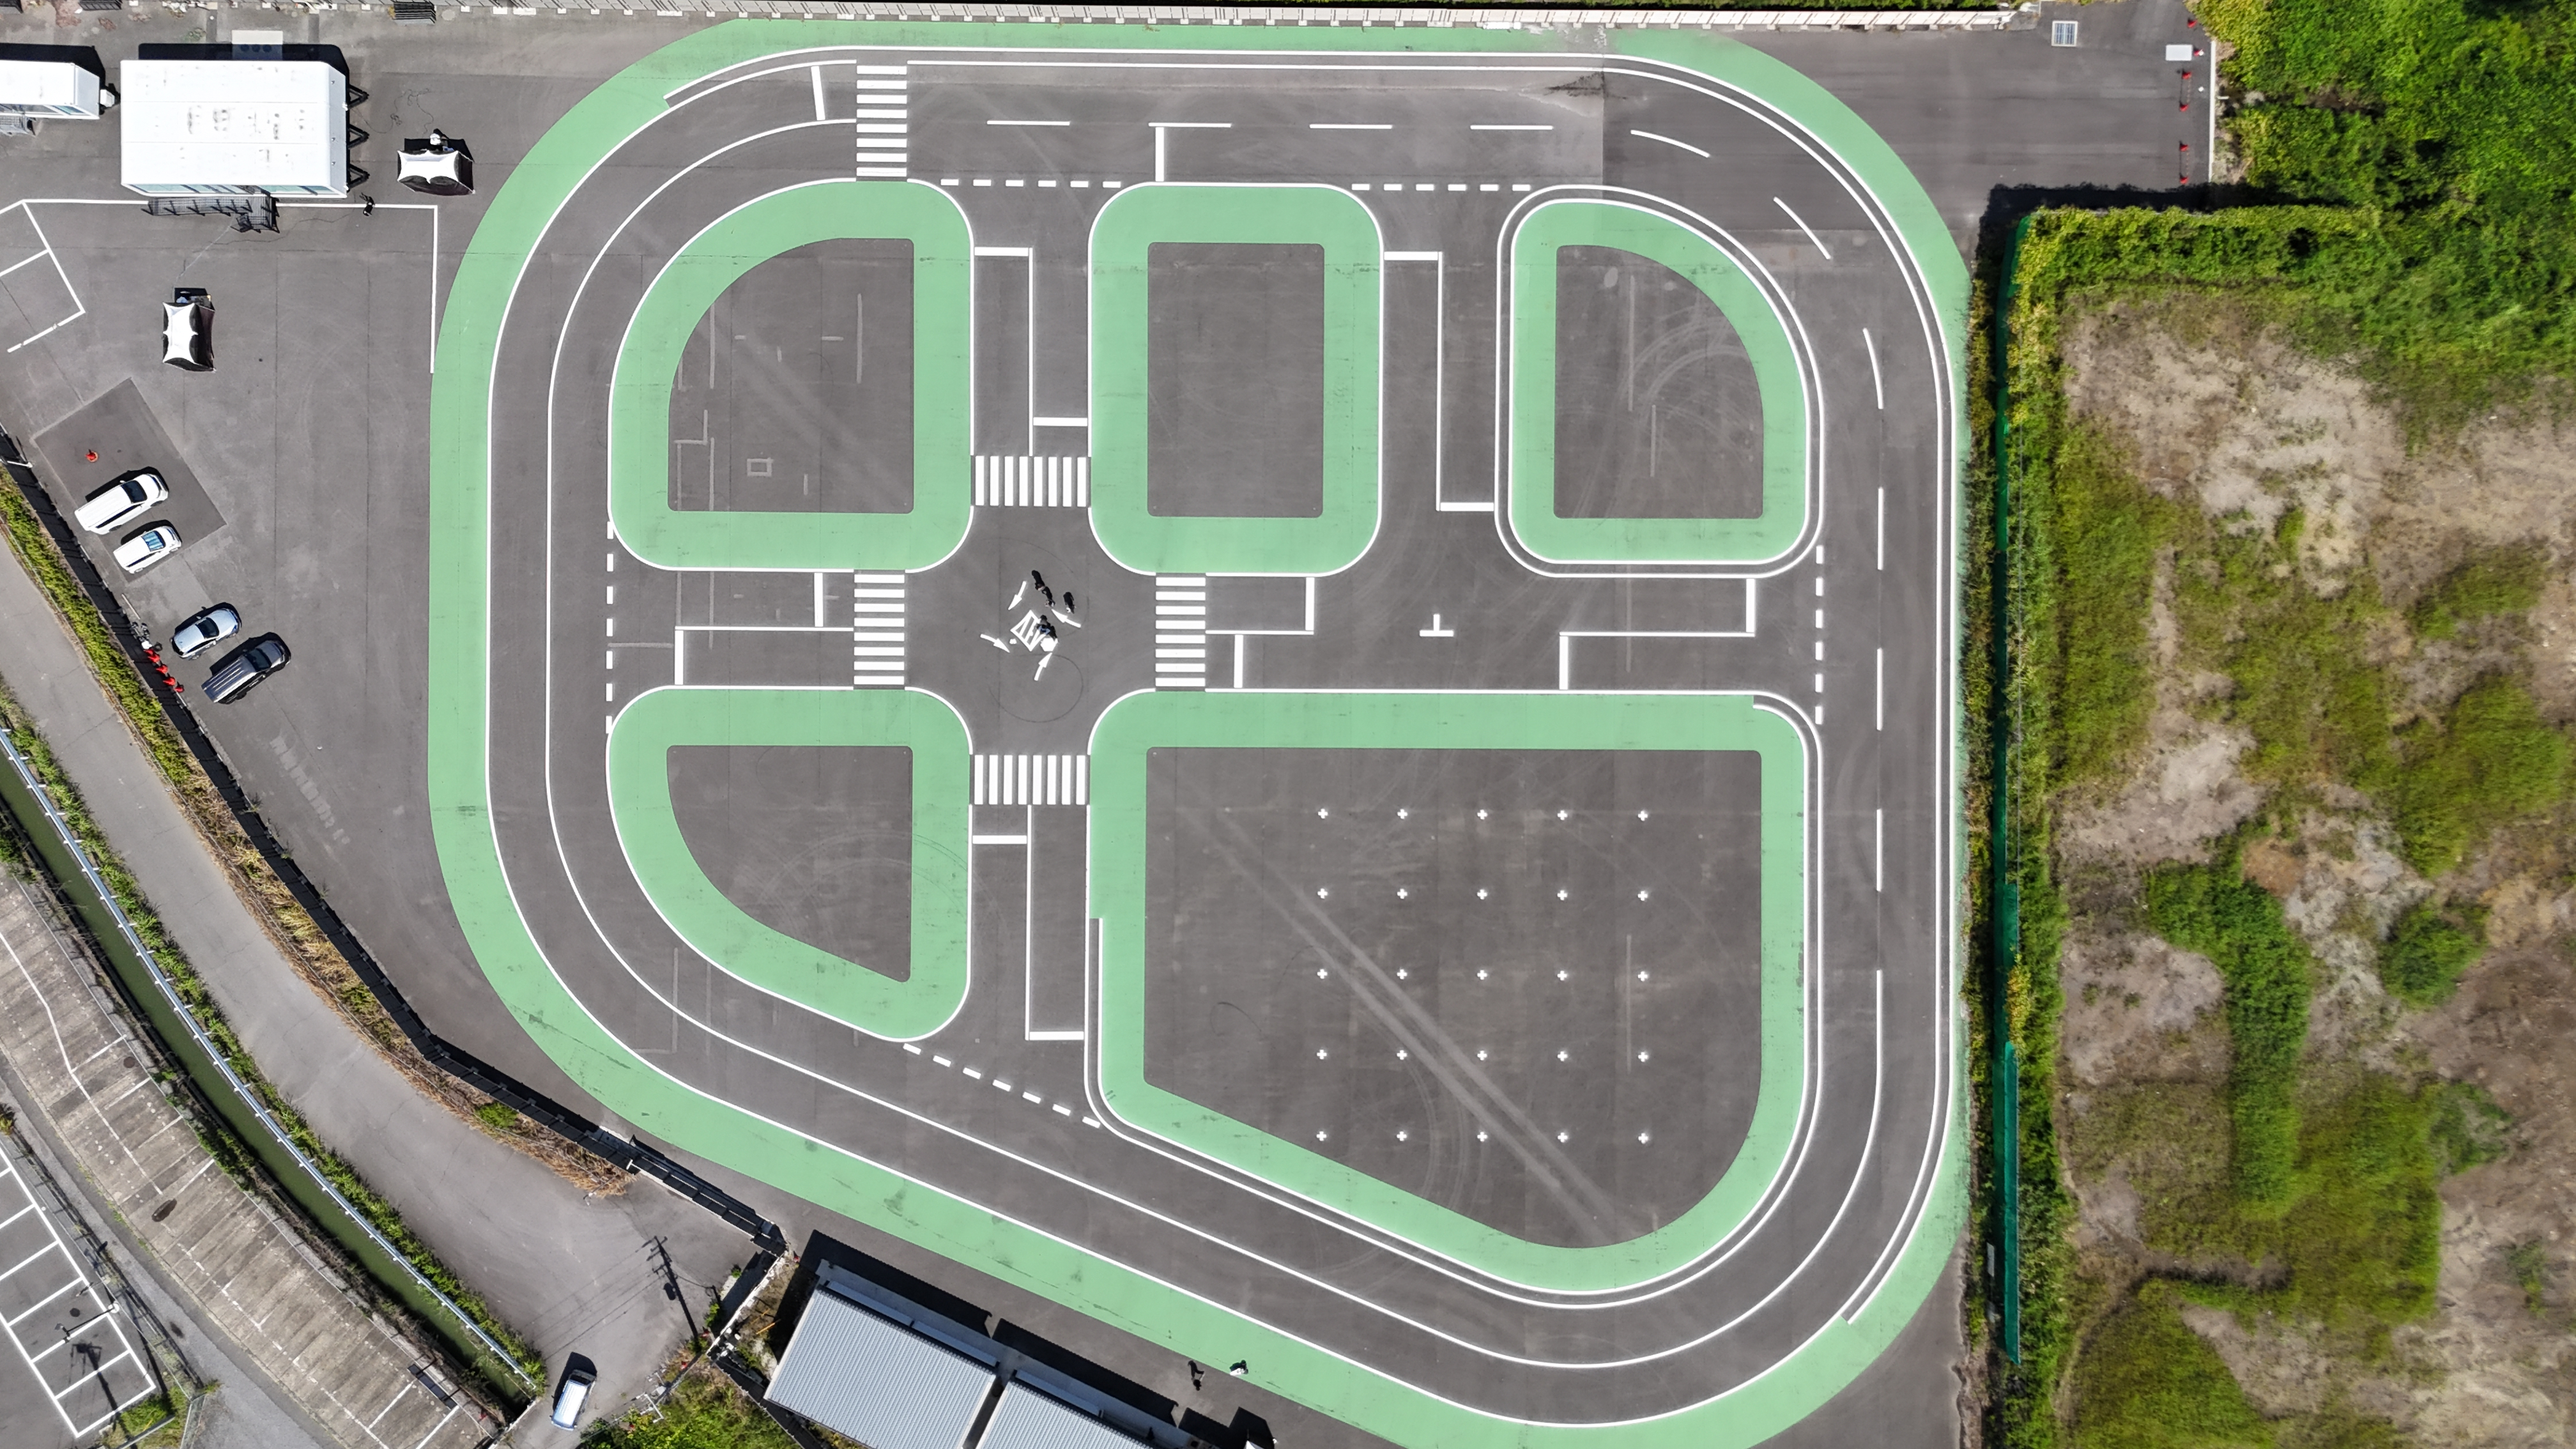
\includegraphics[keepaspectratio, scale=0.1]
      {images/AerialViewAndMobilitysPerspetiveOfTheCourse.png}
 \caption{Aerial view and mobility perspective of the course}
 \label{fig:course}
\end{figure}

\section{実験装置}
本研究で使用する実験装置をFig.6.2に示す.
ハードウェアは, 本田技術研究所から貸与されたロボットを使用する.
このロボットは差動二輪+従動輪で構成された三輪モデルとなっている.
貸与された状態のロボットから従動輪をモータで駆動する形式に変更を加えている.
また, 安全面を考慮してロボットにアンテナを取り付けて遠隔で非常停止ボタンが押せるようにしている.
PCの仕様をTable.6.1に示す.
経路追従にはGNSS+IMUセンサ(VectorNav VN-200)を使用する.
ソフトウェアはROS 2を使用して構築している.

fig(センサに着目したロボットの画像)

本研究で開発した経路追従ソフトウェアは事前に用意した目標経路に沿って追従する動作を行う.
本実験で使用する目標経路は実験日と同日にAIモビリティパークを手動走行させて取得したGNSSデータを基準に作成している.
Fig.6.3に用意した目標経路をGoogle Map上にプロットした図を示す.

\begin{figure}[H]
  \centering
 \includegraphics[keepaspectratio, scale=0.3]
      {images/targetpath.png}
 \caption{Aerial view and mobility perspective of the course}
 \label{fig:course}
\end{figure}

\section{実験内容}
AIモビリティパークで自律走行させることで経路追従の有効性を検証する.
並進速度は3m/sから開始させて, PIDゲインなどのパラメータを調整しながら徐々に並進速度を上げてパラメータチューニングを行った.
実験を行うコースをFig.6.4に示す.
ロボットはFig.6.4の丸で示された位置から矢印に沿うようなルートでコースを一周する.

\begin{figure}[H]
  \centering
 \includegraphics[keepaspectratio, scale=0.6]
      {images/AIFormulapath.png}
 \caption{Experiment path}
 \label{fig:path}
\end{figure}

\newpage

\section{実験結果と考察}

\subsection{実験1}
走行時のパラメータをTable.6.1に示す.
\begin{table}[H]
     \centering
     \caption{experiment1 parameters}
     \begin{tabular}{cclll}
     \multicolumn{1}{c|}{linear\_vel}     & 3.0  &  &  &  \\
     \multicolumn{1}{c|}{interval\_ms}    & 50   &  &  &  \\
     \multicolumn{1}{c|}{lookahead\_gain} & 1.0  &  &  &  \\
     \multicolumn{1}{c|}{p gain}          & 0.8  &  &  &  \\
     \multicolumn{1}{c|}{i gain}          & 0.0  &  &  &  \\
     \multicolumn{1}{c|}{d gain}          & 0.0 &  &  &  \\
     \multicolumn{1}{l}{}                 &      &  &  &  \\
     \multicolumn{1}{l}{}                 &      &  &  & 
     \end{tabular}
\end{table}

実験の結果, 並進速度3m/sでコースを一周することができた.
目標経路に対して大きなズレも無く追従することができることを確認できた.
実験時の走行経路と目標経路の軌跡をFig.6.5に示す.
また, 目標経路との誤差の遷移をFig.6.6に示す.
最後に評価項目の結果をTable.6.2に示す.

\begin{figure}[H]
     \centering
    \includegraphics[keepaspectratio, scale=0.7]
         {images/3mspath.png}
    \caption{Trajectory of travel route and target route}
    \label{fig:path}
\end{figure}

\begin{figure}[H]
     \centering
    \includegraphics[keepaspectratio, scale=0.7]
         {images/3mserror.png}
    \caption{Transition of error from the target path}
    \label{fig:path}
\end{figure}

\begin{table}[H]
     \centering
     \caption{evaluation item}
     \begin{tabular}{cclll}
     \multicolumn{1}{c|}{並進速度{[}m/s{]}}         & 3.0  &  &  &  \\
     \multicolumn{1}{c|}{走行時間{[}s{]}}           & 140?   &  &  &  \\
     \multicolumn{1}{c|}{走行経路と目標経路の累積誤差{[}m{]}} & 2244.0 &  &  &  \\
     \multicolumn{1}{c|}{走行経路と目標経路の最大誤差{[}m{]}} & 2.8 &  &  &  \\
                                                &      &  &  &  \\
                                                &      &  &  &  \\
     \multicolumn{1}{l}{}                       &      &  &  &  \\
     \multicolumn{1}{l}{}                       &      &  &  & 
     \end{tabular}
\end{table}

\subsection{実験2}
走行時のパラメータをTable.6.3に示す.

\begin{table}[H]
     \centering
     \caption{experiment1 parameters}
     \begin{tabular}{cclll}
     \multicolumn{1}{c|}{linear\_vel}     & 6.0  &  &  &  \\
     \multicolumn{1}{c|}{interval\_ms}    & 50   &  &  &  \\
     \multicolumn{1}{c|}{lookahead\_gain} & 1.0  &  &  &  \\
     \multicolumn{1}{c|}{p gain}          & 1.0  &  &  &  \\
     \multicolumn{1}{c|}{i gain}          & 0.0  &  &  &  \\
     \multicolumn{1}{c|}{d gain}          & 0.15 &  &  &  \\
     \multicolumn{1}{l}{}                 &      &  &  &  \\
     \multicolumn{1}{l}{}                 &      &  &  & 
     \end{tabular}
\end{table}

実験の結果, 並進速度6m/sでコースを一周することができた.
コース東側の道で蛇行する動きを見せたものの, 経路から外れることなく周回することができた.
実験時の走行経路と目標経路の軌跡をFig.6.5に示す.
また, 目標経路との誤差の遷移をFig.6.6に示す.
最後に評価項目の結果をTable.6.4に示す.

\begin{figure}[H]
     \centering
    \includegraphics[keepaspectratio, scale=0.7]
         {images/6mspath2.png}
    \caption{Trajectory of travel route and target route}
    \label{fig:path}
\end{figure}

\begin{figure}[H]
     \centering
    \includegraphics[keepaspectratio, scale=0.7]
         {images/6mserror.png}
    \caption{Transition of error from the target path}
    \label{fig:path}
\end{figure}

\begin{table}[H]
     \centering
     \caption{evaluation item}
     \begin{tabular}{cclll}
     \multicolumn{1}{c|}{並進速度{[}m/s{]}}         & 6.0  &  &  &  \\
     \multicolumn{1}{c|}{走行時間{[}s{]}}           & 43   &  &  &  \\
     \multicolumn{1}{c|}{走行経路と目標経路の累積誤差{[}m{]}} & 1130.0 &  &  &  \\
     \multicolumn{1}{c|}{走行経路と目標経路の最大誤差{[}m{]}} & 2.11 &  &  &  \\
                                                &      &  &  &  \\
                                                &      &  &  &  \\
     \multicolumn{1}{l}{}                       &      &  &  &  \\
     \multicolumn{1}{l}{}                       &      &  &  & 
     \end{tabular}
\end{table}
% 7章
\chapter{結論}
%!TEX root = ../thesis.tex
本研究では, AI-Formulaで使用する屋外自律高速モビリティを対象として経路追従行動を行うためのソフトウェア開発を行った.
また, 開発した経路追従ソフトウェアをシミュレータ環境と実環境で検証した.
検証の結果, 予め与えられた目標経路に対して経路追従する動作を確認した.
% シミュレータ環境と実環境で開発した経路追従ソフトウェアを使用し, 経路に追従して目標経路を完走する行動を確認した.